%++++++++++++++++++++++++++++++++++++++++
\documentclass[a4paper,11pt]{article}
\usepackage{url}
\usepackage{hyperref}
\usepackage{fullpage}
\usepackage{booktabs}
\usepackage{graphicx}
\usepackage{wrapfig}
\usepackage{caption}
\usepackage{float}
\usepackage{subcaption}
\usepackage{enumerate}
\usepackage{color}
\usepackage{capt-of}
\usepackage{todonotes}
\usepackage{geometry}
 \geometry{
   a4paper,
   total={170mm,257mm},
   left=15mm,
   right=15mm,
   top=15mm,
 }
\usepackage{indentfirst}
  \setlength{\parindent}{0.5em}
  \setlength{\parskip}{0.1em} 
\usepackage{tabularx} % extra features for tabular environment
\usepackage{amsmath}  % improve math presentation
\newcommand{\Test}[1]{\expandafter\hat#1}
\usepackage{graphicx} % takes care of graphic including machinery
\hypersetup{
    colorlinks=true,       % false: boxed links; true: colored links
    linkcolor=blue,        % color of internal links
    citecolor=blue,        % color of links to bibliography
    filecolor=magenta,     % color of file links
    urlcolor=blue
}

% other packages
\usepackage{listings} % code listings
\lstset{framextopmargin=0pt,frame=lines}
\lstset{
    basicstyle=\footnotesize\ttfamily,
    breaklines=true,
    tabsize=4,
    keepspaces=true,
    columns=flexible,
    % backgroundcolor=\color[gray]{0.9},
    frame=single
}
\lstset{language=Matlab,%
    %basicstyle=\color{red},
    breaklines=true,%
    morekeywords={matlab2tikz},
    keywordstyle=\color{blue},%
    morekeywords=[2]{1}, keywordstyle=[2]{\color{black}},
    identifierstyle=\color{black},%
    stringstyle=\color{mylilas},
    commentstyle=\color{mygreen},%
    showstringspaces=false,%without this there will be a symbol in the places where there is a space
    numbers=left,%
    numberstyle={\tiny \color{black}},% size of the numbers
    numbersep=9pt, % this defines how far the numbers are from the text
    emph=[1]{for,end,break},emphstyle=[1]\color{red}, %some words to emphasise
    %emph=[2]{word1,word2}, emphstyle=[2]{style},    
}
\usepackage{color} %red, green, blue, yellow, cyan, magenta, black, white
\definecolor{mygreen}{RGB}{28,172,0} % color values Red, Green, Blue
\definecolor{mylilas}{RGB}{170,55,241}

\usepackage{todonotes}
\usepackage[toc,page]{appendix}

%++++++++++++++++++++++++++++++++++++++++

\begin{document}



\title{
    System Identification \\
    CE-3: Parametric Identification Methods
}
\author{Camilla Carta \\ Michael Spieler}
\date{\today}
\maketitle

\section{Identification of a laser beam stabilizing system}

For the first part of this exercise the objective was to identify a parametric model for a laser beam stabilizing system, as shown in Figure \ref{fig:systlaserbeam}.

\begin{figure}[H]
\centering
\includegraphics[height = 4cm]{images/laserbeamsystem}
\caption{Laser beam stabilizing system}
\label{fig:systlaserbeam}
\end{figure}

The datafile \texttt{laserbeamdataN.mat} contained the experimental data coming from the system: 

\begin{itemize}
\item the input signal \texttt{u} which is a PRBS;
\item the output signal \texttt{y}, which is the beam position;
\item a sampling period of $T_e = 0.001s$.
\end{itemize}

In order to identify an optimal parametric model, different models were studied.

\subsection{FIR model identification}
First, a finite impulse response model was studied.

Let's assume that the output of the system depends only on past inputs:
\begin{equation}
y(k) = b_1u(k-1) + b_2u(k-2) + ... + b_mu(k-m)
\end{equation}
Then, the $z$-tranform will give
\begin{equation}
Y(z)=(b_1z^{-1} + b_2z^{-2} + ... + b_mz^{-m})U(z) = G(z)U(z)
\end{equation}
Now, the output of the FIR model can be predicted by
\begin{equation}
\hat{y}(k,\theta) = \phi^T(k)\theta
\end{equation}
where
\begin{equation}
\phi^T(k)=[u(k-1),u(k-2),...,u(k-m)] 
\end{equation}

\begin{equation}
\theta^T = [b_1,b_2,...,b_m]
\end{equation}

The code for the application of this method can be found in Appendix \ref{app:ce3_2}. The vector of parameters $\theta^T = [b_1,...,b_m]$ found can be observed in Figure \ref{fig:est_theta_FIR}, while its covariance can be seen in Figure \ref{fig:cov_FIR}.
Finally, the predicted output can be compared to the real output (see Figure \ref{fig:y_FIR}).



\begin{figure}[H]
\centering
\begin{subfigure}[t]{0.4\textwidth}
\centering
\includegraphics[height = 4cm]{images/theta_FIR}
\caption{Estimated values of parameters $b$}
\label{fig:est_theta_FIR}
\end{subfigure}
~
\begin{subfigure}[t]{0.4\textwidth}
\centering
\includegraphics[height = 4cm]{images/cov_FIR}
\caption{Covariance of the estimates with a $\pm2\sigma$}
\label{fig:cov_FIR}
\end{subfigure}
\caption{Estimated values of theta and their covariance for FIR method with m=50}
\label{fig:theta_FIR}
\end{figure}

\begin{figure}[H]
\centering
\includegraphics[height = 6cm]{images/y_FIR}
\caption{Real output against estimated FIR output}
\label{fig:y_FIR}
\end{figure}

It can be observed that the estimation is quite satisfactory In order to evaluate the performance of the predictor, the loss function can be used, as explained in the course notes at page 109. As such, it can be calculated as $J(\hat{\theta})/N$, with

\begin{equation}
J(\hat{\theta}) = \sum\limits_{k=1}^N(y(k)-\hat{y}(k))
\end{equation}

where $J(\hat{\theta})$ is the fit criterion. In this case, the loss function was equal to $1.3854\cdot10^{-8}$. Nevertheless, the number of parameters was limited at $m=50$, while m should be theoretically infinite in order to perfectly represent the system. 


\subsection{ARX model identification}
The second model that was studied was a second order ARX model, given by the following predictor:
\begin{equation}
\hat{y}(k,\theta) = -a_1y(k-1)-a_2y(k-2) + b_1u(k-1) + b_2u(k-2) = \phi^T(k)\theta
\end{equation}

As in the course notes (pp. 71-72), it can be demonstrated that the parameters can be identified using the least square algorithm, which gives
\begin{equation}
\hat{\theta} = \left[ \sum\limits_{k=1}^N \phi(k)\phi^T(k)\right]^{-1}\left[ \sum\limits_{k=1}^N \phi(k)y(k)\right]
\end{equation}
with
\begin{equation}
\phi^T(k)=[-y(k-1),-y(k-2),u(k-1),u(k-2)]
\end{equation}
and
\begin{equation}
\theta^T=[a_1,a_2,b_1,b_2]
\end{equation}

The code application can be found in Appendix ref\ref{app:ce3_3}. 

The estimated model was found to be
\begin{equation}
\hat{y}(k)=1.5483y(k-1)-0.6484y(k-2)+0.0183u(k-1)+0.0731u(k-2)
\end{equation}

The results for the output prediction and the output for the identified model compared to the real output can be seen in Figure \ref{fig:ARX_outputs}. In particular, it can be observed in Figure \ref{fig:yhat_ARX} that the prediction is close to the real output. The loss function, computed as above, was equal to $4.3396\cdot10^{-8}$, while the 2-norm of the output error was equal to $1.066782\cdot10^{-2}$ when compared to the output corresponding to this simulation (see Figure \ref{fig:ym_ARX}). We notice that the simulated output behaves much worse than the predicted output.


\begin{figure}[H]
\centering
\begin{subfigure}[t]{0.4\textwidth}
\centering
\includegraphics[height = 5cm]{images/yhat_ARX}
\caption{Real output against predicted ARX output}
\label{fig:yhat_ARX}
\end{subfigure}
~
\begin{subfigure}[t]{0.4\textwidth}
\centering
\includegraphics[height = 5cm]{images/ym_ARX}
\caption{Real output against the output for the ARX model}
\label{fig:ym_ARX}
\end{subfigure}
\caption{Real output compared to ARX prediction and modeled output}
\label{fig:ARX_outputs}
\end{figure}

\subsection*{Instrumental Variable method}
In order to have unbiased parameter estimated for the ARX model, the vector of instrumental variables can be used, as shown at page 74 for the course notes. As such, the new estimate will be

\begin{equation}
\hat{\theta_{iv}}=\left[ \sum\limits_{k=1}^N \phi(k)\phi^T(k)\right]^{-1}\left[ \sum\limits_{k=1}^N \phi_{iv}(k)y(k)\right]
\end{equation}
where $\phi(k)$ remains unchanged and $\phi_{iv}^T(k)$ is declared as
\begin{equation}
\phi_{iv}^T(k)=[-y_M(k-1),...-y_M(k-n),u(k-d-1),...,u(k-d-m)]
\end{equation}
and the noiseless output of this model as
\begin{equation}
y_M(k)=M(q^{-1})u(k)
\end{equation}

This new model gave a loss function of $2.2195\cdot10^{-7}$ and an output error of $4.696157\cdot10^{-3}$, which means this model has less precise prediction than the ARX model, but its simulated output is improved. The results can be seen in Figure \ref{fig:IV_outputs}.


\begin{figure}[H]
\centering
\begin{subfigure}[t]{0.4\textwidth}
\centering
\includegraphics[height = 5cm]{images/yhat_IV}
\caption{Real output against predicted IV output}
\label{fig:yhat_IV}
\end{subfigure}
~
\begin{subfigure}[t]{0.4\textwidth}
\centering
\includegraphics[height = 5cm]{images/ym_IV}
\caption{Real output against the output for the IV model}
\label{fig:ym_IV}
\end{subfigure}
\caption{Real output compared to IV prediction and modeled output}
\label{fig:IV_outputs}
\end{figure}




\subsection{State-space model identification}

The general form of a state-space model is

\begin{equation}
\begin{split}
x(k+1)=Ax(k)+Bu(k)+w(k) \\
y(k)=Cx(k)+Du(k)+e(k)
\end{split}
\end{equation}

Following the course notes at pages 78-80, an estimation of the parameters A, B and C can be computed. In particular, 

\begin{equation}
Y_r(k)=\begin{bmatrix}
y(k)\\
y(k+1)\\
\vdots \\
y(k+r-1)
\end{bmatrix} , 
U_r=\begin{bmatrix}
u(k)\\
u(k+1)\\
\vdots \\
u(k+r-1)
\end{bmatrix}
\end{equation}

\begin{equation}
\textbf{Y} = [Y_r(1),Y_r(2),...,Y_r(N)]
\end{equation}

\begin{equation}
\textbf{U} = [U_r(1),U_r(2),...,U_r(N)]
\end{equation}

\begin{equation}
\textbf{U}^{\perp}=\textbf{I}-\textbf{U}^T(\textbf{UU}^T)^{-1}\textbf{U}
\end{equation}
\begin{equation}
\textbf{Q}=\textbf{YU}^{\perp} = O_r\textbf{XU}^{\perp}
\end{equation}

As stated in the course notes, the rank of the matrix $\textbf{Q}$ should estimate the order of the system. However, in presence of noise, the rank can over-estimate the order: as such, one should compute the singular values and choose the most representative number. Indeed, the \verb'svd' command was used to find the results shown in Figure \ref{fig:Q_svd}. It can be observed that the singular values tend towards 0 for all orders higher than 2. The maximum order n was then chosen equal to 2.
The r parameter was then optimized by recursive iteration, that tested for values from 1 to 20. As can be seen in Figure \ref{fig:r}, the optimum loss function was found to be for $r=9$.

\begin{figure}[H]
\centering
\begin{subfigure}[t]{0.4\textwidth}
\centering
\includegraphics[height = 6cm]{images/Q_svd}
\caption{Singular values for the augmented observability matrix}
\label{fig:Q_svd}
\end{subfigure}
~
\begin{subfigure}[t]{0.4\textwidth}
\centering
\includegraphics[height = 6cm]{images/r}
\caption{Loss function in function of r}
\label{fig:r}
\end{subfigure}
\caption{Optimisation of n and r parameters}
\label{fig:optimize_nr}
\end{figure}

Subsequently, an estimation of the observability matrix $O_r$ could be constructed by taking the first n columns and the first r rows of \textbf{Q}. Then, $\hat{C}$ can be estimated as the first $n_y$ row of $O_r$ and $\hat{A}$ can be computed from the equation

\begin{equation}
[\textnormal{the last $(r-1)n_y$ rows of $O_r$} ]=[\textnormal{the first $(r-1)n_y$ rows of $O_r$} ] \times \hat{A}
\end{equation}

The identified parameters are
\begin{equation}
\hat{A}=\begin{bmatrix}
0.2655 &  -1.0140 \\
0.3648 &  1.3732
\end{bmatrix}
 ,
 \hat{C} =10^{-3}\cdot\begin{bmatrix}
 0.3767 &  -0.0184
 \end{bmatrix}
\end{equation}

From these parameters, the estimations for B could be computed as well, by using the least square algorithm 
\begin{equation}
\hat{y}(k)=\hat{C}(qI-\hat{A})^{-1}Bu(k)+Du(k)=u_f(k)B
\end{equation}
where
\begin{equation}
u_f(k)=\hat{C}(qI-\hat{A})^{-1}u(k) ~\textnormal{and}~\hat{D}=0
\end{equation}

$\hat{B}$ was then computed as
\begin{equation}
\hat{B}= (U_f^TU_f)U_f^TY=\begin{bmatrix}
10.2157\\
 -286.7666
\end{bmatrix}
\end{equation}

Finally, the measured output was compared to the state-space model found (see Figure \ref{fig:ym_SSID}). The 2-norm error was equal to $5.846650\cdot10^{-3}$.

\begin{figure}[H]
\centering
\includegraphics[height = 6cm]{images/ym_SSID}
\caption{Measured output compared to state-space model output}
\label{fig:ym_SSID}
\end{figure}


\section{Parametric Identification of a Flexible Link}

For the second part the objective was to identify a parametric black-box model for a rotary flexible link, as shown in Figure \ref{fig:syst}.

\begin{figure}[H]
\centering
\includegraphics[height = 4cm]{images/system}
\caption{Flexible link system}
\label{fig:syst}
\end{figure}

We were provided with following data:
\begin{itemize}
\item the input signal \texttt{u} which is a PRBS of length N=2000 which consists of 4 periods.
\item the output signal \texttt{y}, which is the link deflection measured by a strain gauge.
\item a sampling period of $T_e = 0.015s$.
\end{itemize}

Before all, we normalize the data using the \verb'detrend' MATLAB function to remove the DC component of the measurements.

\subsection{Order estimation}
The MATLAB code for the order estimation can be found in Appendix \ref{app:ce3_5}.

\subsubsection{Manual order estimation using ARX}
Using the \verb'arx' command 10 models of orders from 1 to 10 with $n_k = 1$ and $n_a = n_b = n = 1..10$ were identified and the loss function, which is shown in Figure \ref{fig:arxlossfn}, was calculated for each model. By hand we estimated an order of $n=6$ (which corresponds to the manually chosen threshold of 0.002 represented by the horizontal red line in Figure \ref{fig:arxlossfn}). Beyond order 6 the loss function stops decreasing significantly.

\begin{figure}[H]
\centering
\includegraphics[width=0.4\textwidth]{images/arxordsel}
\caption{ARX order selection}
\label{fig:arxlossfn}
\end{figure}

\subsubsection{Order estimation using ARMAX with zero/pole cancellation}
The order can be estimated by identifying multiple ARMAX models and plotting the zeros/poles with their confidence intervals. When the confidence intervals of a zero/pole pair intersects, then it can be assumed that they cancel each other out. Thus zero/pole cancellation should occur above the true order n, which we observe for orders above $n=7$ (shown in Figure \ref{fig:zeropolecancel}). It is thus verified that this is very close to the order $n=6$ estimated above. Therefore we choose the order $n=7$. 

\begin{figure}[H]
\centering
\includegraphics[width=\textwidth]{images/zeropolecancel}
\caption{Additional zeros/poles cancel each other out for order $n>7$.}
\label{fig:zeropolecancel}
\end{figure}


\subsubsection{Estimate the delay}
To estimate the delay $n_k$ we identify first an ARX system with $n_a = n_b = 7$ and $n_k = 0$.
Then the parameters $b_1 to b_m$ of B were studied and the first $n_k$ coefficients of B that are close to zero were determined.
Due to noise, the coefficients are not exactly 0 and thus the confidence interval of the estimated coefficients $b_i$ is studied, as shown in Figure \ref{fig:nksel}. If the 0 lies in the confidence interval then the parameter $b_i$ is considered to be close to zero.
Thus we find $n_k = 2$.

\begin{figure}[H]
\centering
\includegraphics[width=0.5\textwidth]{images/nksel}
\caption{Order selection using ARX}
\label{fig:nksel}
\end{figure}

\subsubsection{Estimation using \texttt{selstruc} command}
Finally, MATLAB's \verb'selstruc' command was used to estimate the parameters $n_a$, $n_b$ and $n_k$. Figure \ref{fig:selstruc} shows the output. Akaike Information Criterion (AIC) estimate was discarded as an overestimated model order ($n_a=9$, $n_b=10$ and $n_k=1$). Therefore we select by hand the number of parameters as 12, $n_a=6$, $n_b=6$ and $n_k=3$. This result is close to the values obtained above.

\begin{figure}[H]
\centering
\includegraphics[width=0.8\textwidth]{images/selstruc}
\caption{Order estimation using selstruc}
\label{fig:selstruc}
\end{figure}

\subsection{Parametric identification and validation}

We divided the data in two equal parts of length N=1000, one for identification and one for validation.

We identify 6 different parametric models for our system using following MATLAB methods:
\begin{itemize}
\item \verb'arx' for ARX structure
\item \verb'iv4' for Instrumental Variables method
\item \verb'armax' for ARMAX structure
\item \verb'oe' for Output-Error structure
\item \verb'bj' for Box-Jenkins structure
\item \verb'n4sid' for State-space structure
\end{itemize}

with following parameters: 
\begin{itemize}
\item $n_a = n_b = 6$
\item $n_k = 3$ delay
\item $n_c = n_d = n_a$ for structures with noise model
\item $n_f = n_a$ for Box-Jenkins structure
\item $n_x = n_a$ for State-space structure
\end{itemize}
The MATLAB code for the parametric identification can be found in Appendix \ref{app:ce3_5_2}.


The results are shown in Figure \ref{fig:syst_compare}. We observe that the Box-Jenkins structure has the best fit  (95.6\%) followed by ARMAX (90.6\%). This is not surprising, since they are the most complex structures with the highest number of parameters. 

The models were validated by the whiteness test of the residuals and the cross-correlation of the residuals with the \verb'resid' MATLAB command (see Figures \ref{fig:syst_resid1} and \ref{fig:syst_resid2}). It can be observed that the best results are given by the Box-Jenkins and the ARMAX models, which validates their performance. 

Although the ARMAX is slightly less performing than the Box-Jenkins, its validation is slightly better. Moreover, it is slightly less complex than the Box-Jenkins.
For these reasons, it is the preferred model in this case.

\begin{figure}[H]
\centering
\includegraphics[width=\textwidth]{images/ce3_5_2_system_compare}
\caption{Comparison between the systems and the validation data: the plots display the normalized root mean square measure of the fit in percentage}
\label{fig:syst_compare}
\end{figure}

\begin{figure}[H]
\centering
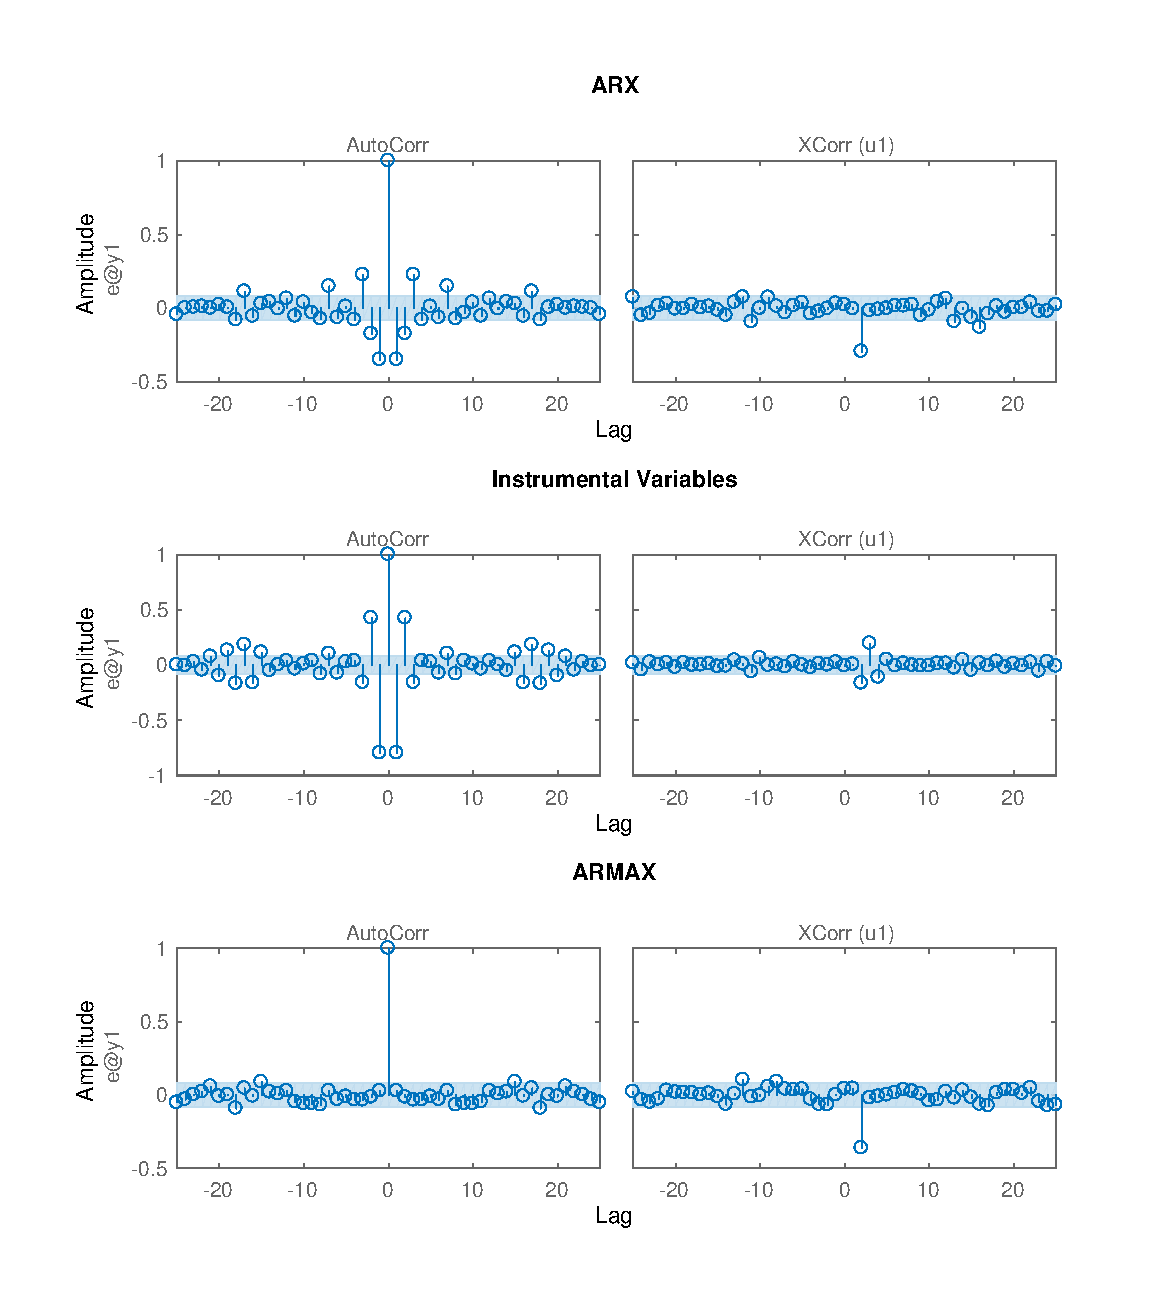
\includegraphics[width=\textwidth]{images/ce3_5_2_system_resid1}
\caption{Auto-correlation of the residuals and their cross-correlation with the input signals for ARX, IV and ARMAX. The 99\% confidence region marking statistically insignificant correlations is also shown as a patch around the plot X-axis}
\label{fig:syst_resid1}
\end{figure}

\begin{figure}[H]
\centering
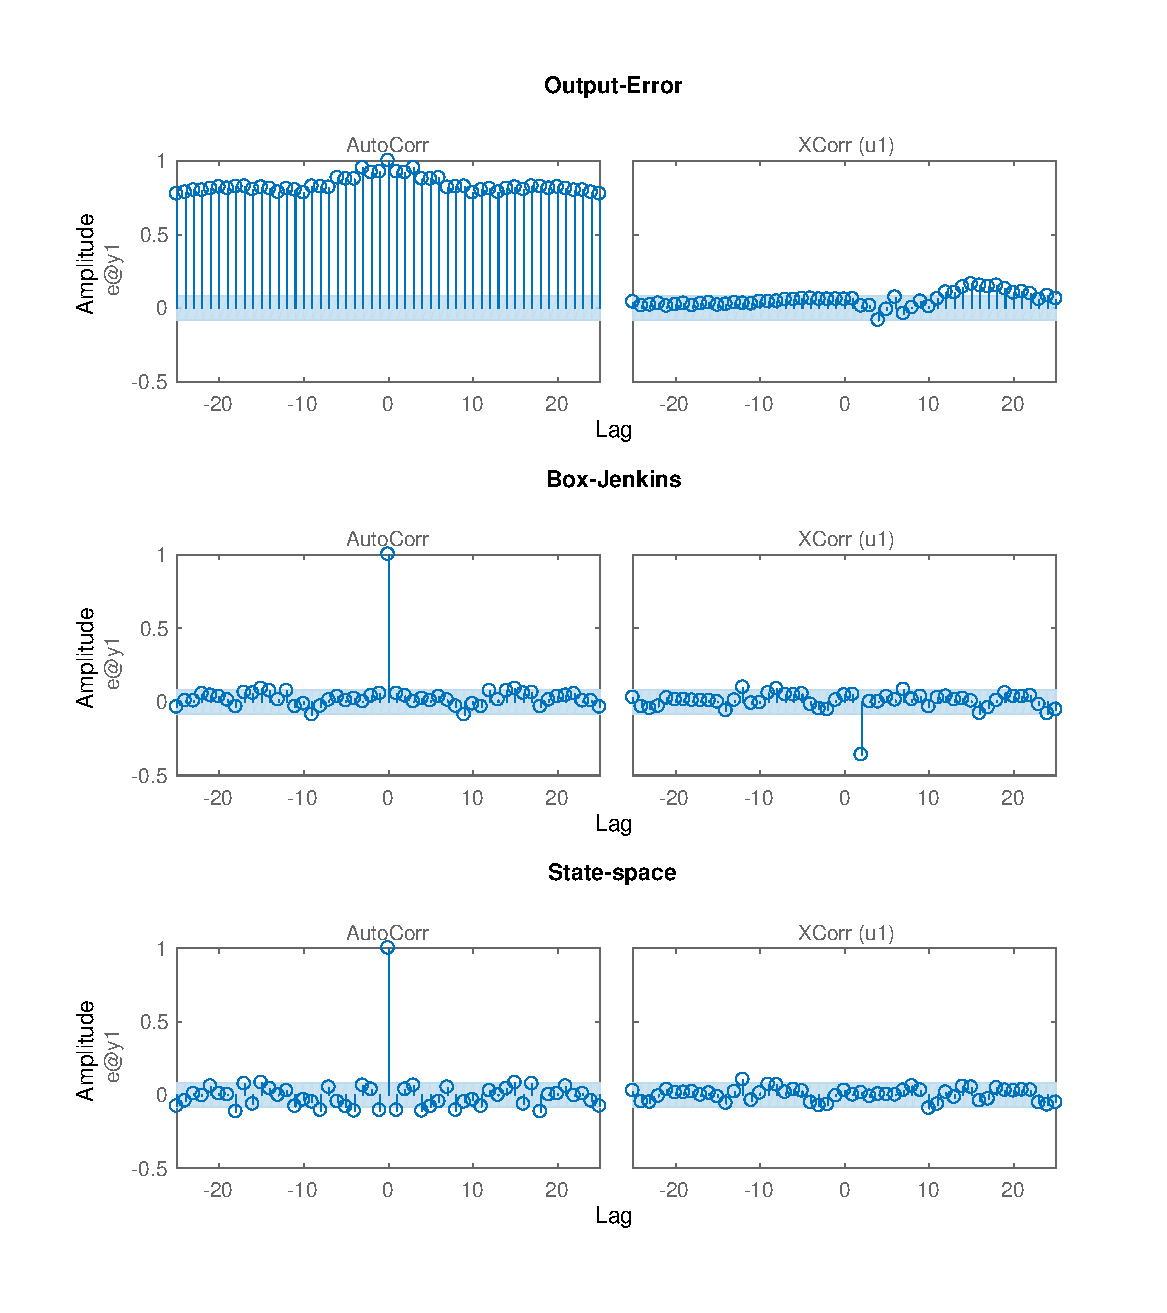
\includegraphics[width=\textwidth]{images/ce3_5_2_system_resid2}
\caption{Auto-correlation of the residuals and their cross-correlation with the input signals for OE, BJ and SSID. The 99\% confidence region marking statistically insignificant correlations is also shown as a patch around the plot X-axis}
\label{fig:syst_resid2}
\end{figure}

The Output-Error structure does not pass the whiteness test since $R_{\epsilon\epsilon}(h) \neq 0$ for $\forall h \neq 0$, which was not expected.


\begin{appendices}
\section{ce3\_2.m}
\label{app:ce3_2}
\lstinputlisting{ce3_2.m}

\section{ce3\_3.m}
\label{app:ce3_3}
\lstinputlisting{ce3_3.m}

\section{ce3\_4.m}
\label{app:ce3_4}
\lstinputlisting{ce3_4.m}

\section{ce3\_5.m}
\label{app:ce3_5}
\lstinputlisting{ce3_5.m}

\section{ce3\_5\_2.m}
\label{app:ce3_5_2}
\lstinputlisting{ce3_5_2.m}

\end{appendices}

\end{document}
